\documentclass{article}
\usepackage{multirow}
\usepackage{graphicx}
\title{Exercise 5\\System On Chip}
\author{Ole Magnus Ruud\\Vegar K\aa sli}
\begin{document}
\maketitle{}
\section{Scenarios}
\begin{center}
  \begin{tabular}{|r|p{8cm}|}
    \hline
\multicolumn{2}{|c|}{Use case scenario 1}\\\hline
Name:&Successful search for the right button order\\\hline
Context:&Top-level mode\\\hline
Pre-conditions:&Memory Machine is in initial state, no lights lit\\\hline
Post-conditions:&All lights are lit\\\hline
Start/Trigger:&User pushes a button\\\hline
Actors:&User, Memory Machine\\\hline
Description:&The user tries out pushing several buttons until one is lit. She then
    tries pushing another button causing the light to go out. She remembers
    the button that lit the first light and pushes this again, trying another
    second button. This time it is the right one, and the user continues in this
    fashion until she finds the complete correct button sequence and all the lights
    are lit\\\hline

  \end{tabular}
\end{center}


\begin{center}
  \begin{tabular}{|r|p{8cm}|}
    \hline
\multicolumn{2}{|c|}{Use case scenario 2}\\\hline
Name:&Unsuccessful search for the right button order\\\hline
Context:&Top-level mode\\\hline
Pre-conditions:&Memory Machine is in initial state, no lights\\\hline
Post-conditions:&No lights are lit\\\hline
Start/Trigger:&User pushes a button\\\hline
Actors/Roles:&User, Memory Machine\\\hline
Description:&
    The user tries out pushing several buttons until one is lit. He then
    tries pushing another button causing the light to go out. He remembers 
    the button that lit the first light and pushes this again, trying another
    second button. This time it is the right one, and he tries one more button
    which causes the lights to go out. This time he fails to remember the 
    first two buttons, and his frustration makes him give up.\\\hline

  \end{tabular}
\end{center}
\section{Sequence diagrams}
\begin{center}
  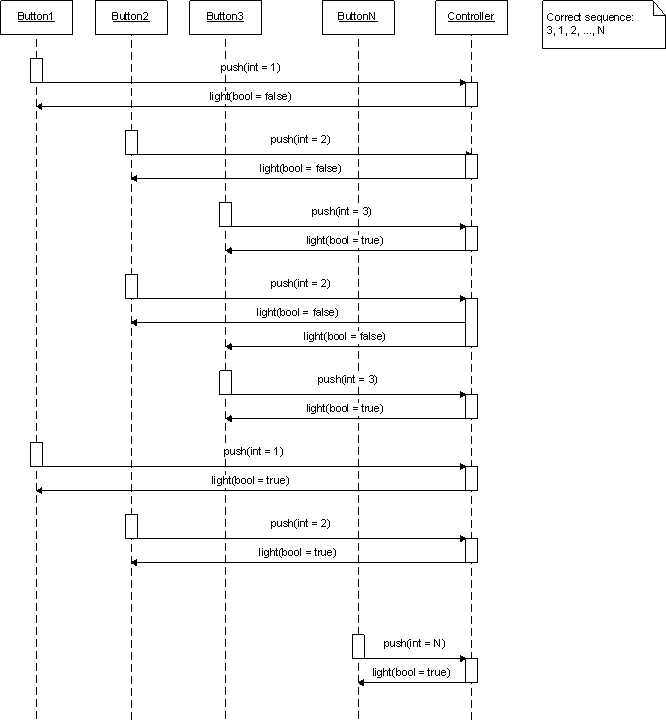
\includegraphics[width=\linewidth]{../sequence_scenario1}
  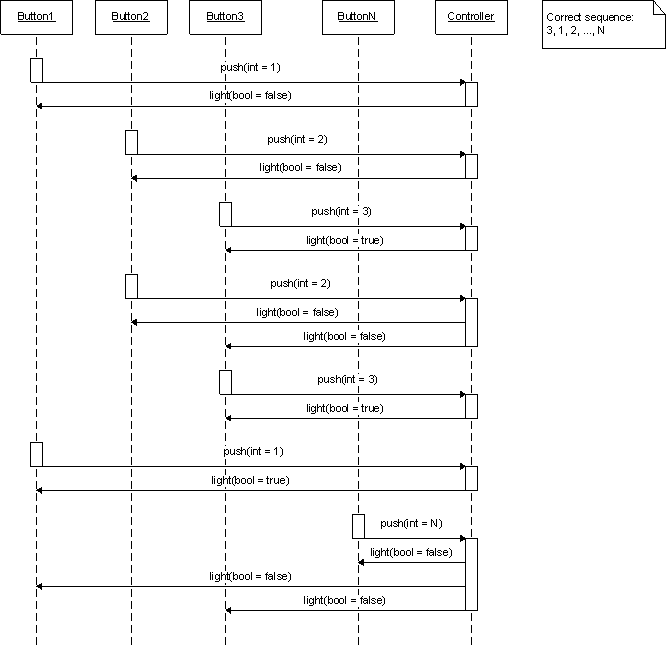
\includegraphics[width=\linewidth]{../sequence_scenario2}

\end{center}
\section{Class, objects and collaborations}
  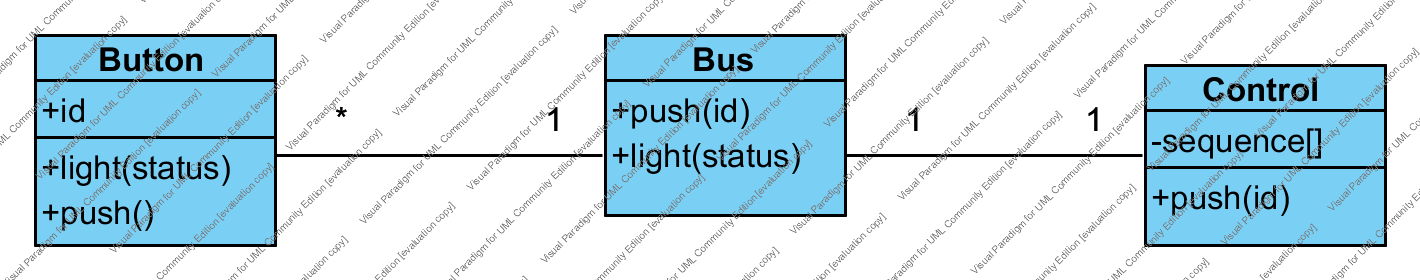
\includegraphics[width=\linewidth]{../class1}
  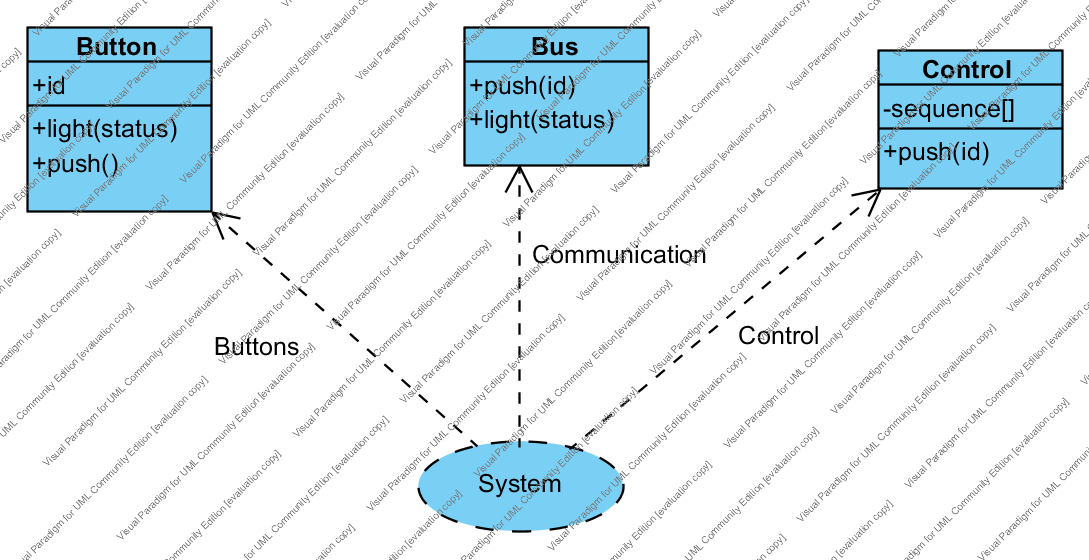
\includegraphics[width=\linewidth]{../class2}
  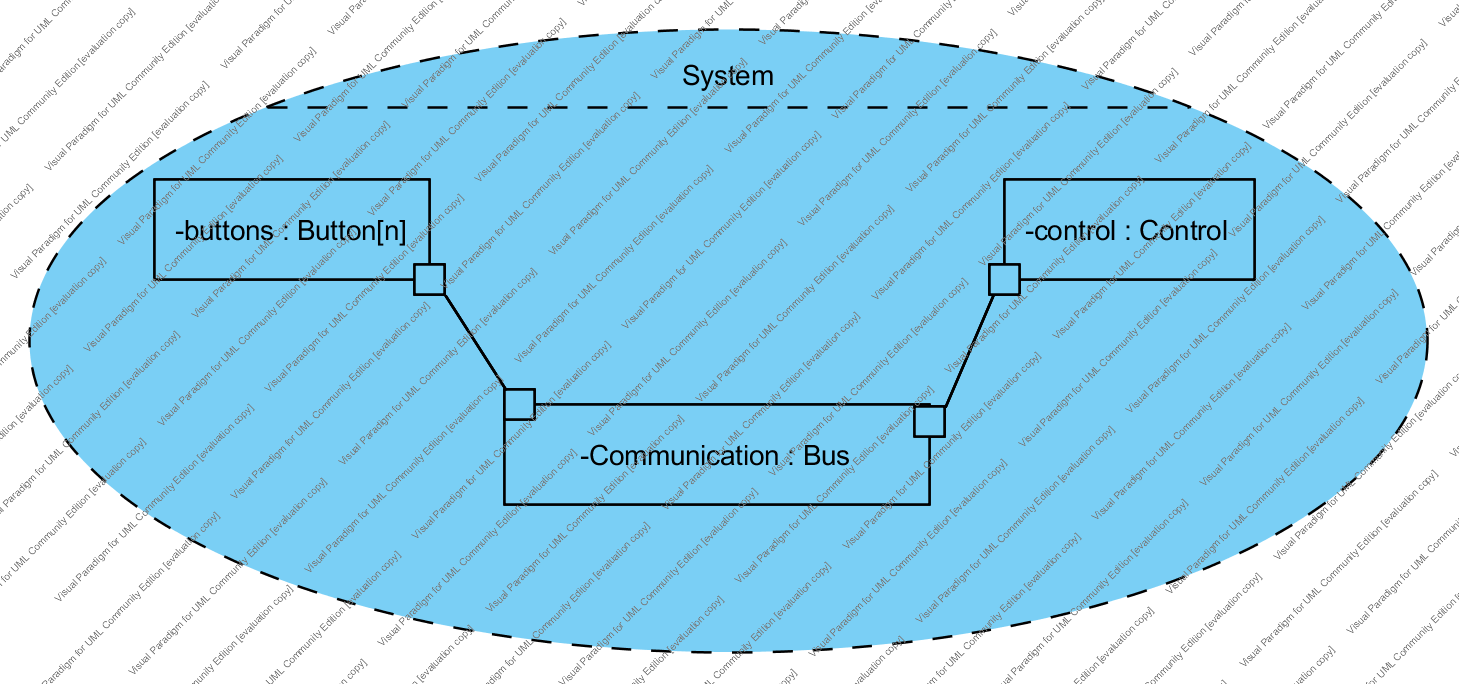
\includegraphics[width=\linewidth]{../comp1}
  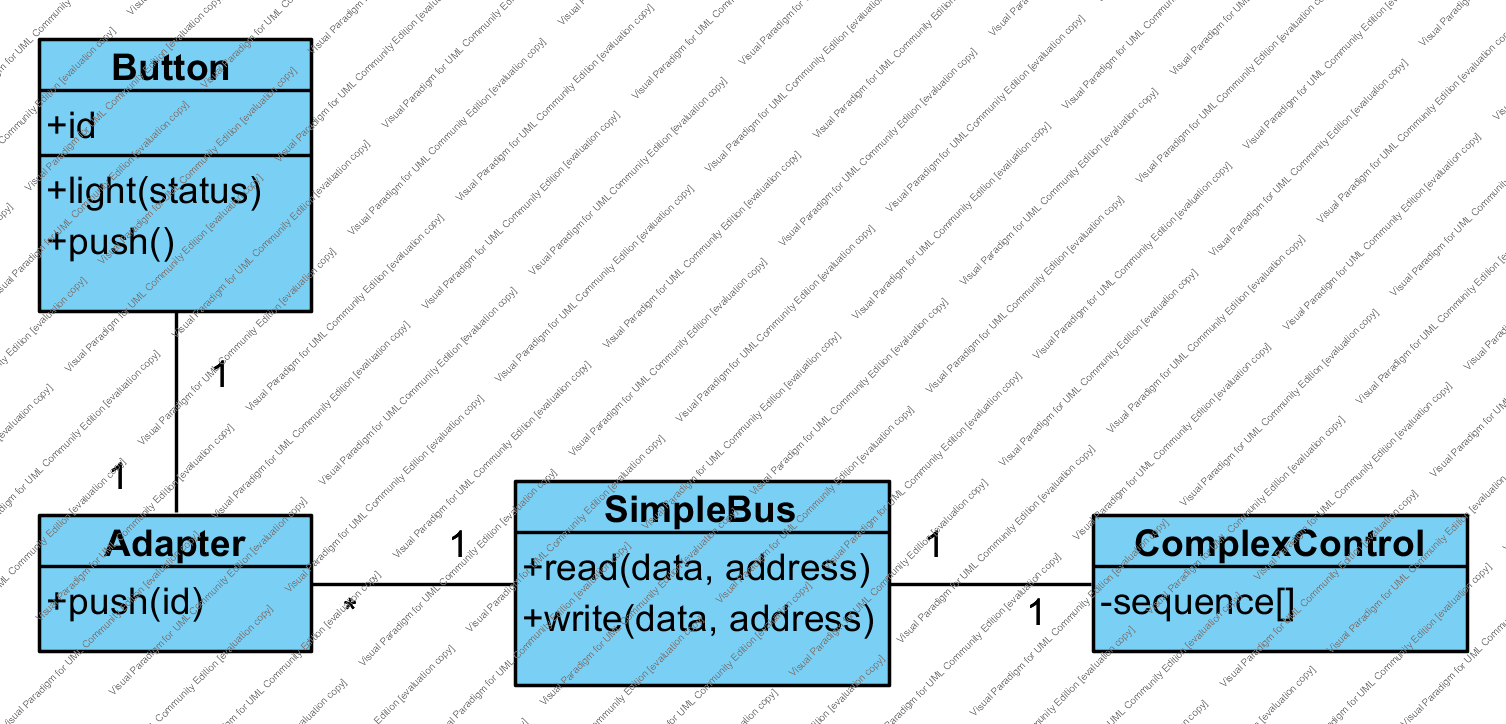
\includegraphics[width=\linewidth]{../class3}
  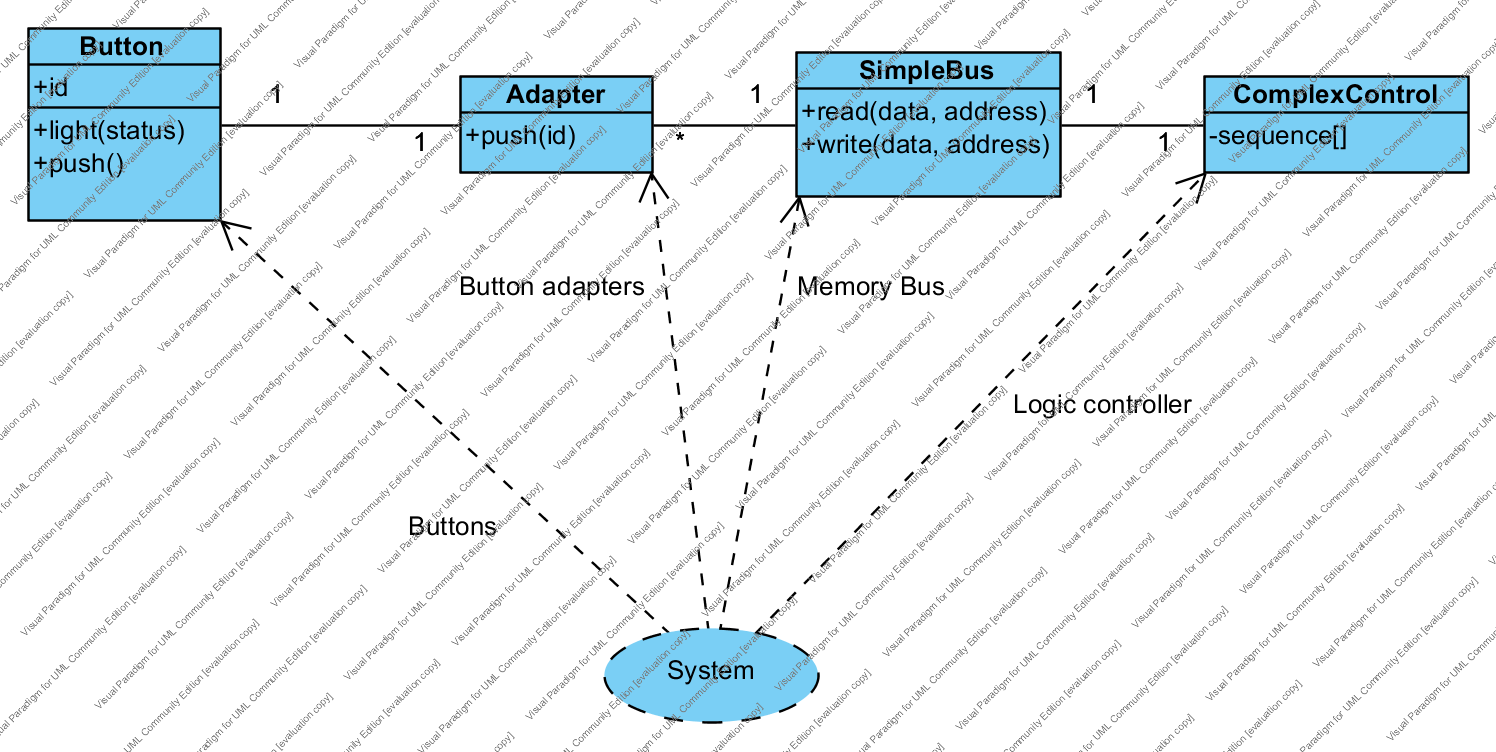
\includegraphics[width=\linewidth]{../class4}
  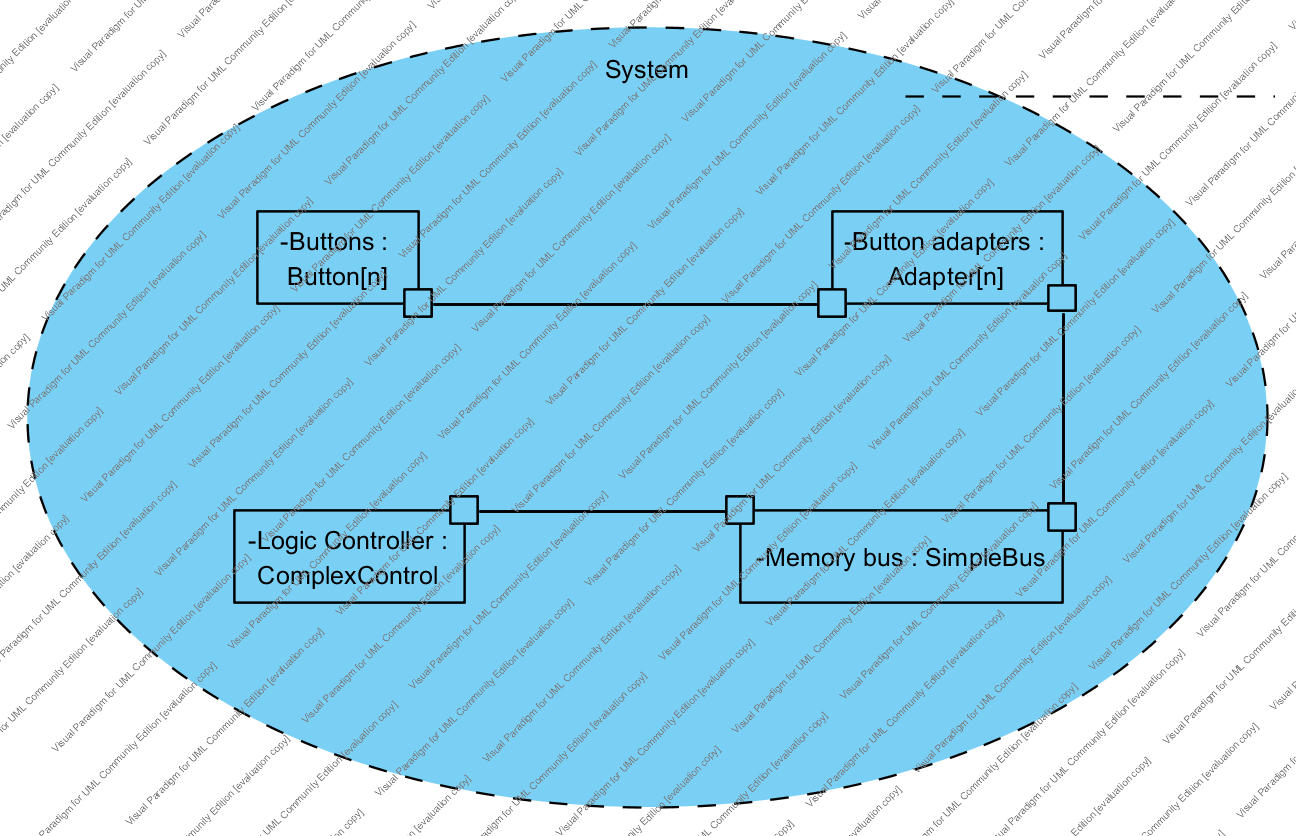
\includegraphics[width=\linewidth]{../comp2}


\section{State Machine Diagrams}


\end{document}
